\documentclass[11pt, a4paper, leqno]{article}
\usepackage{a4wide}
\usepackage[T1]{fontenc}
\usepackage[utf8]{inputenc}
\usepackage{float, afterpage, rotating, graphicx}
\usepackage{epstopdf}
\usepackage{longtable, booktabs, tabularx}
\usepackage{fancyvrb, moreverb, relsize}
\usepackage{eurosym, calc}
% \usepackage{chngcntr}
\usepackage{amsmath, amssymb, amsfonts, amsthm, bm}
\usepackage{caption}
\usepackage{mdwlist}
\usepackage{xfrac}
\usepackage{setspace}
\usepackage[dvipsnames]{xcolor}
\usepackage{subcaption}
\usepackage{minibox}
% \usepackage{pdf14} % Enable for Manuscriptcentral -- can't handle pdf 1.5
% \usepackage{endfloat} % Enable to move tables / figures to the end. Useful for some
% submissions.

\usepackage[
    natbib=true,
    bibencoding=inputenc,
    bibstyle=authoryear-ibid,
    citestyle=authoryear-comp,
    maxcitenames=3,
    maxbibnames=10,
    useprefix=false,
    sortcites=true,
    backend=biber
]{biblatex}
\AtBeginDocument{\toggletrue{blx@useprefix}}
\AtBeginBibliography{\togglefalse{blx@useprefix}}
\setlength{\bibitemsep}{1.5ex}
\addbibresource{refs.bib}

\usepackage[unicode=true]{hyperref}
\hypersetup{
    colorlinks=true,
    linkcolor=black,
    anchorcolor=black,
    citecolor=NavyBlue,
    filecolor=black,
    menucolor=black,
    runcolor=black,
    urlcolor=NavyBlue
}


\widowpenalty=10000
\clubpenalty=10000

\setlength{\parskip}{1ex}
\setlength{\parindent}{0ex}
\setstretch{1.5}


\begin{document}

\title{EXAMPLE PROJECT}
\thanks{EXAMPLE UNIVERSITY. Email: janedoe[at]example-university.de}

\author{JANE DOE}

\date{
    {\bf Preliminary -- please do not quote}
    \\[1ex]
    \today
}

\maketitle


\begin{abstract}
    Some abstract here.
\end{abstract}

\clearpage


\section{Introduction} % (fold)
\label{sec:introduction}

If you are using this template, please cite this item from the references:
\citet{GaudeckerEconProjectTemplates}.

The data set for the template project is taken from
\url{https://www.stem.org.uk/resources/elibrary/resource/28452/large-datasets-stats4schools}.
It contains data on smoking habits in the UK, with 1691 observations and 12 variables.
We consider only 4 of the 12 features for the prediction of the variable
\texttt{smoking}: \texttt{marital\_status}, \texttt{highest\_qualification},
\texttt{gender} and \texttt{age}. We model the dependence using a Logistic model. All
numerical features are included linearly, while categorical features are expanded into
dummy variables. Figures below illustrate the model predictions over the lifetime. You
will find one figure and one estimation summary table for each installed programming
language.


\begin{figure}[H]

    \centering
    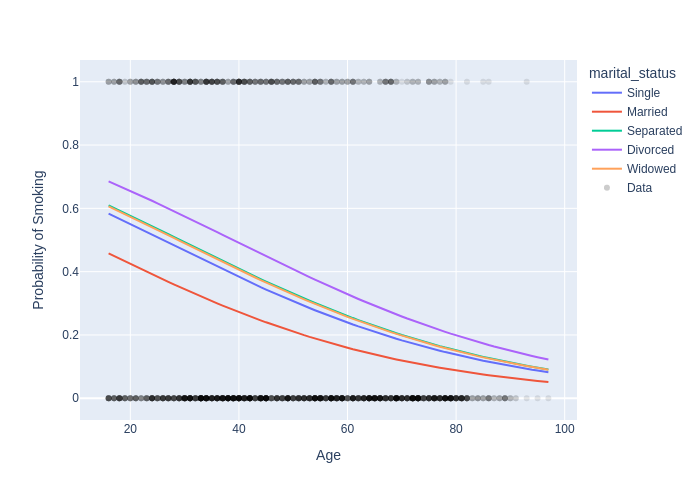
\includegraphics[width=0.85\textwidth]{../figures/smoking_by_marital_status}

    \caption{Model predictions of the smoking probability over the lifetime. Each
        colored line represents a case where marital status is fixed to one of the
        values present in the data set.}
    \label{fig:predictions}

\end{figure}


\begin{table}[!h]
    \begin{center}
\begin{tabular}{lclc}
\toprule
\textbf{Dep. Variable:}                                           & current\_smoker\_numerical & \textbf{  No. Observations:  } &     1691    \\
\textbf{Model:}                                                   &           Logit            & \textbf{  Df Residuals:      } &     1679    \\
\textbf{Method:}                                                  &            MLE             & \textbf{  Df Model:          } &       11    \\
\textbf{Date:}                                                    &      Thu, 17 Apr 2025      & \textbf{  Pseudo R-squ.:     } &  0.08598    \\
\textbf{Time:}                                                    &          08:55:10          & \textbf{  Log-Likelihood:    } &   -867.39   \\
\textbf{converged:}                                               &            True            & \textbf{  LL-Null:           } &   -948.98   \\
\textbf{Covariance Type:}                                         &         nonrobust          & \textbf{  LLR p-value:       } & 2.961e-29   \\
\bottomrule
\end{tabular}
\begin{tabular}{lcccccc}
                                                                  & \textbf{coef} & \textbf{std err} & \textbf{z} & \textbf{P$> |$z$|$} & \textbf{[0.025} & \textbf{0.975]}  \\
\midrule
\textbf{Intercept}                                                &       0.8786  &        0.255     &     3.443  &         0.001        &        0.378    &        1.379     \\
\textbf{gender[T.Male]}                                           &       0.1776  &        0.122     &     1.455  &         0.146        &       -0.062    &        0.417     \\
\textbf{marital\_status[T.Married]}                               &      -0.5050  &        0.157     &    -3.220  &         0.001        &       -0.812    &       -0.198     \\
\textbf{marital\_status[T.Separated]}                             &       0.1102  &        0.292     &     0.378  &         0.706        &       -0.462    &        0.682     \\
\textbf{marital\_status[T.Divorced]}                              &       0.4419  &        0.216     &     2.050  &         0.040        &        0.019    &        0.864     \\
\textbf{marital\_status[T.Widowed]}                               &       0.0970  &        0.269     &     0.360  &         0.719        &       -0.431    &        0.625     \\
\textbf{highest\_qualification[T.GCSE/CSE or GCSE/O Level]}       &      -0.1076  &        0.168     &    -0.642  &         0.521        &       -0.436    &        0.221     \\
\textbf{highest\_qualification[T.ONC/BTEC]}                       &      -0.3583  &        0.292     &    -1.228  &         0.220        &       -0.930    &        0.214     \\
\textbf{highest\_qualification[T.Other/Sub or Higher/Sub Degree]} &      -0.2999  &        0.192     &    -1.560  &         0.119        &       -0.677    &        0.077     \\
\textbf{highest\_qualification[T.A Levels]}                       &      -0.9393  &        0.288     &    -3.266  &         0.001        &       -1.503    &       -0.376     \\
\textbf{highest\_qualification[T.Degree]}                         &      -1.1184  &        0.218     &    -5.139  &         0.000        &       -1.545    &       -0.692     \\
\textbf{age}                                                      &      -0.0339  &        0.005     &    -7.120  &         0.000        &       -0.043    &       -0.025     \\
\bottomrule
\end{tabular}
%\caption{Logit Regression Results}
\end{center}

    \label{tab:summary}
    \caption{Estimation results of the linear Logistic regression.}
\end{table}



\setstretch{1}
\printbibliography
\setstretch{1.5}


% \appendix

% The chngctr package is needed for the following lines.
% \counterwithin{table}{section}
% \counterwithin{figure}{section}

\end{document}
